\documentclass{article}

\usepackage{amsmath, mathtools, amsthm}
\usepackage{graphicx}
\graphicspath{ {./} }

\title{Prima guerra mondiale}
\author{github.com/asdrubalini}
\date{\today}

\begin{document}
\maketitle

\section{Le cause dello scoppio della guerra}
Le cause che hanno contribuito a scatenare la prima guerra mondiale si possono suddividere in quattro categorie:

\begin{center}
    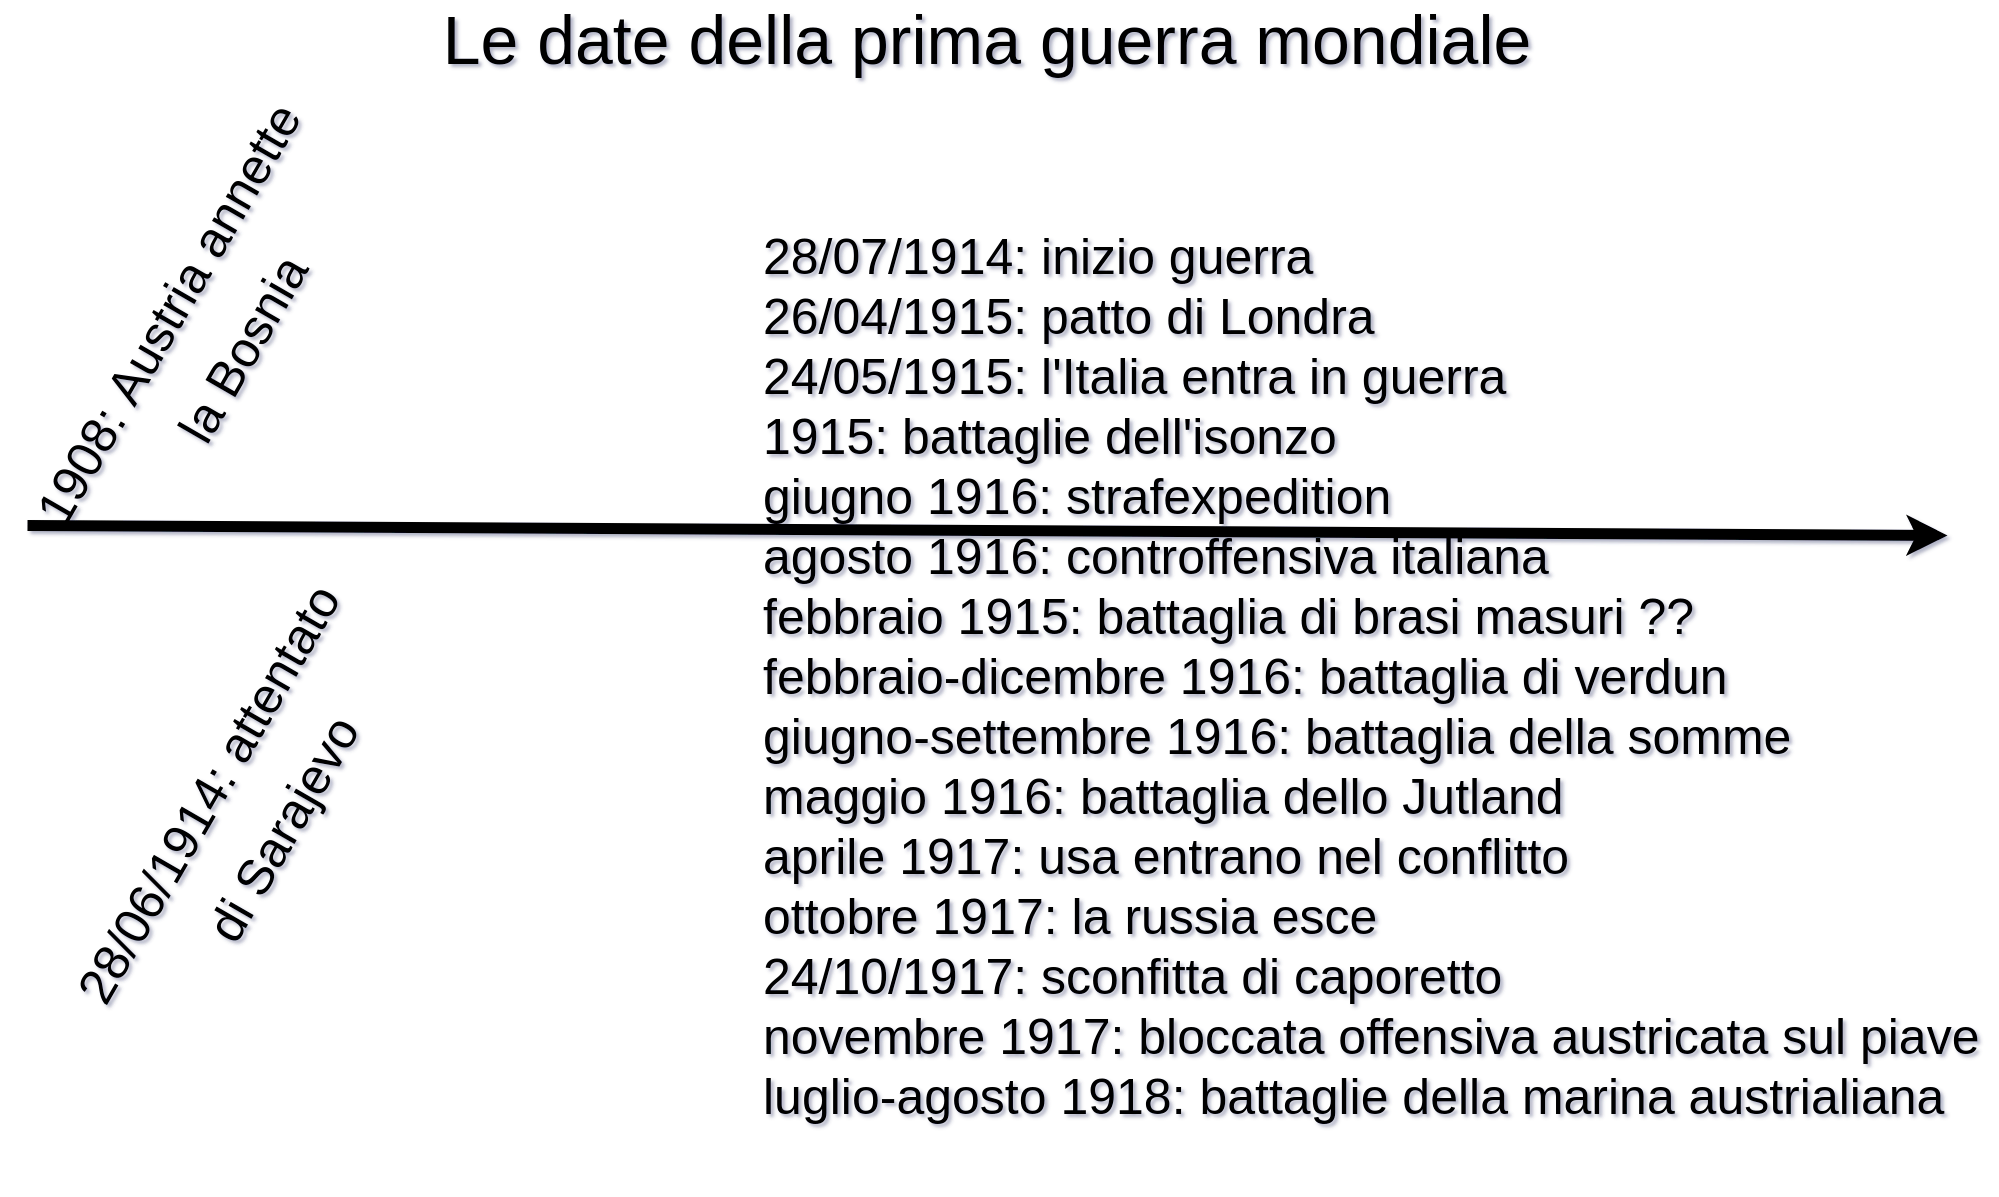
\includegraphics[width=\textwidth]{date.png}
\end{center}

\subsection{Cause politiche}
\begin{enumerate}
    \item Germania voleva diventare prima potenza mondiale al posto dell'inghilterra;
    \item La Francia voleva prendersi la rivincita contro la Germania;
    \item Crisi dell'impero ottomano: gli altri stati volevano espandersi. La prima a farlo fu l'Austria;
    \item La presenza di due blocchi militari contrapposti: triplice alleanza (Germania, Austria, Italia) e triplice intesa (Gran Bretagna, Francia e Russia).
\end{enumerate}

\subsection{Cause economiche}
\begin{enumerate}
    \item Rivalità tra le colonie da parte delle potenze industriali.
\end{enumerate}

\subsection{Cause militari}
\begin{enumerate}
    \item Corsa agli armamenti spinta dai gruppi industriali.
\end{enumerate}

\subsection{Cause culturali}
\begin{enumerate}
    \item Nazionalismo: volontà di affermare la propria nazione sulle altre;
    \item Applicazione del Darwinismo: la guerra decide le nazioni che dominano;
    \item I giovani borghesi volevano affermarsi grazie alla guerra;
    \item Futurismo, la guerra era la sola igiene del mondo.
\end{enumerate}

\subsection{Lo scoppio della guerra}

Il 28 Giugno 1914 l'arciduca Francesco Ferdinando, erede al trono Austriaco, viene assassinato da un ragazzo Serbo durante
l'attentato di Sarajevo.
L'Austria chiede alla Serbia di consegnargli l'assassino, tuttavia la Serbia è costretta a rifiutare poichè aveva
stretto un accordo con la Russia.\\
Un mese dopo, il 28 Luglio 1914, inizia la guerra.

\begin{itemize}
    \item Austria
    \item Germania
    \item Turchia
    \item Bulgaria
\end{itemize}

contro

\begin{itemize}
    \item Serbia
    \item Russia
    \item Francia
    \item Inghilterra
    \item Italia
    \item Stati Uniti
\end{itemize}

Inizialmente si pensa ad una guerra lampo per via delle nuove tecnologie, tuttavia così non fu.\\
\newline
L'Italia si divide in due fazioni: neutralisti ed interventisti.
\newline

Neutralisti:
\begin{itemize}
    \item Opinione pubblica;
    \item Liberali giolittiani (Giolitti credeva che l'Italia non fosse preparata per una guerra. Era convinto che la guerra sarebbe
          durata a lungo);
    \item Cattolici;
    \item La maggior parte dei socialisti.
\end{itemize}

Interventisti:
\begin{itemize}
    \item Nazionalisti;
    \item Irredentisti (volevano l'unificazione dell'Italia e la liberazione delle terre sotto il dominio Austriaco.
          Pensavano che la guerra sarebbe finita in tre o quattro mesi);
    \item Industriali;
    \item Una piccola parte dei socialisti.
\end{itemize}

\section{L'Italia entra in guerra}

Il 26 Aprile 1915 l'Italia entra in guerra con il patto di Londra, a fianco delle potenze dell'Intesa (Inghilterra, Russia e Francia).
In caso di vittoria, l'Italia avrebbe ottenuto diversi territori.\\
Il 24 Maggio 1915 l'Italia abbandona l'alleanza difensiva con la triplice alleanza per dichiarare guerra all'Austria con
il comandante Luigi Cadorna (famoso per la sua disciplina ferrea), anche se non era preparata ad un conflitto.


\subsection{Sabato 12 Febbraio 2022}
L'Italia non era assolutamente preparata ad affrontare un conflitto. L'armamento era pieno di carenze e c'era una forte diversità nelle zone d'Italia. Si trovano a combattere insieme contadini del sud e operai del nord.
\\
Luigi Cadorna era un comandante molto rigido. Disciplina Militare. Si diffonde le fucilazioni in caso di diserzione. Se un soldato prova a scappare viene fucilato. Per quanto riguarda i reati collettivi, si diffonde la pratica della decimazione. 10 uomini venivano estratti a sorte e venivano uccisi.
\\
Fronti della guerra: 4 <slide teams>
\\
Il generale Cadorna tenta un attacco centrale contro l'Austria che porta a migliaia di vittime e nessun territorio.
Gli Austriaci interpretano l'entrata in guerra dell'Italia come un tradimento, nonostante in teoria non lo fosse.

Principali battaglie:
\begin{enumerate}
    \item Battaglia delle Somme
    \item Battaglia dello Jutland
\end{enumerate}

STORIA:
Sono seduti in un campo di papaveri nel fronte occidentale e stanno giocando a carte quando arriva una lettera dal professore che li aveva invogliati ad andare in guerra. Un loro amico si è ferito gravemente ad una gamba ed è in ospedale.

\section{Domande}

\subsection{Quali sono le cause che hanno portato allo scoppio della Prima Guerra Mondiale? E qual è la causa scatenante?}
Il 28 Giugno 1914 l'arciduca Francesco Ferdinando viene assassinato a Sarajevo da un cittadino Serbo, Unito al fatto che
la Serbia non volle collaborare e rifiutò l'ultimatum, l'Austria ebbe la scusa perfetta per poter dichiarare guerra
alla Serbia.\\
Le vere cause però furono la rivalità tra nazioni, l'irredentismo, la questione balcanica, il nazionalismo ed un clima culturale
favorevole alla guerra.

\subsection{Perchè la Serbia respinge l'ultimatum Austriaco?}
L'ultimatum Austriaco era molto umiliante per la Serbia, inoltre avrebbe rotto l'accordo preesistente con la Russia.
La Serbia provò ad accettare solo alcune richieste, tuttavia per l'Austria non fu sufficiente e dichiarò quindi guerra
alla Serbia.

\subsection{La Germania era tenuta ad entrare in guerra a fianco dell'Austria? Perchè lo fa?}
L'alleanza che la Germania aveva con l'Austria era solo di tipo difensivo, per cui la Germania non aveva nessun obbligo
di entrare nel conflitto. Tuttavia, decise comunque di entrare dichiarando guerra alla Russia ed alla Francia per via
di un piano strategico che stava seguendo. Secondo il suddetto piano, la Germania avrebbe dovuto sconfiggere la Francia
in una guerra lampo per poi gestire la situazione russa.

\subsection{Perchè si parla di "guerra di posizione"?}
Inizialmente si pensava che l'invenzione dei veicoli aerei avrebbe rivoluzionato il modo di combattere la guerra,
tuttavia così non fu e la guerra divenne una logorante guerra di posizione dove i soldati passavano settimane
e settimane nelle trincee conquistando e poi perdendo metri di territorio.

\subsection{La situazione in Italia: chi erano i neutralisti e gli interventisti?}
Tra i neutralisti c'è l'opinione pubblica, i liberali Giolittiani, i cattolici e la maggior parte dei socialisti. Tra gli
interventisti, ovvero coloro che volevano entrare in guerra c'erano i nazionalisti, gli irredentisti (ovvero coloro che
avrebbero voluto avere le terre sotto il dominio austriaco), gli industriali ed una piccola parte dei socialisti.

\subsection{Cos'è il Patto di Londra?}
Il Patto di Londra è stato un accordo segreto firmato il 26 Aprile 1915 tra l'Italia e la triplice intesa, secondo il quale
l'Italia sarebbe entrata in guerra un mese dopo in cambio di alcuni territori (Trieste, Gorizia, Istria, Dalmazia, ecc.),
che però non furono completamente riconosciuti.

\subsection{Quando e come l'Italia entra in guerra?}
L'Italia dichiara guerra all'Austria il 24 Maggio 1915, entrando nel conflitto a fianco delle potenze della Triplice intesa
(Inghilterra, Russia e Francia). L'entrata in guerra dell'Italia, che faceva parte anche della triplice alleanza (insieme a
Germania ed Austria-Ungheria), viene vista come un tradimento, nonostante l'alleanza fosse esclusivamente difensiva e
l'Austria aveva invece attaccato.

\subsection{Quali sono le principali battaglie del 1915-16 sul fronte italiano?}
\begin{itemize}
    \item Giugno-Dicembre 1915: Battaglie dell'Isonzo. Il generale Cadorna prova un attacco contro gli Austriaci ma fu un fallimento;
    \item Giugno 1916: Strafexpedition. Spedizione punitiva degli Austriaci contro gli Italiani, l'attacco Russo arresta l'offensiva;
    \item Agosto 1916: controffensiva italiana, liberazione di Gorizia.
\end{itemize}

\subsection{Principali battaglie sugli altri fronti}
\begin{itemize}
    \item Battaglia dei Laghi Masuri, esercito russo viene sconfitto
    \item Battaglia di Verdun, i francesi riescono a resistere
    \item Battaglia della Somme
    \item Battaglia dello Jutland, portò al blocco navale inglese.
\end{itemize}

\subsection{Spiega l'entrata degli USA nel conflitto}
Nel 1917 si pensava che la guerra fosse quasi conclusa, tuttavia il 6 Aprile 1917 gli Stati Uniti decidono di entrare nel
conflitto dalla parte degli alleati in seguito all'affondamento della nave Lusitania da parte delle forze tedesche.

\subsection{Spiega l'uscita della Russia dal conflitto}
Nel 1917, la Russia decide di uscire dal conflitto per via di alcuni problemi interni, più nello specifico la rivoluzione
d'Ottobre di Lenin, che desiderava una guerra tra classi, non un conflitto mondiale con altre potenze. Firmò quindi il
trattato di Brest-Litovsk con la Germania in cui cede l'Ucraina (voluta per i campi coltivati) e portò all'indipendenza
di Ucraina, Finlandia, Estonia, Lettonia, Lituania, Bielorussia e Polonia.

\subsection{Cos'è la sconfitta di Caporetto?}
La battglia di Caporetto è ricordata ancora oggi come una delle più grandi sconfitte della storia italiana. Il fronte infatti
fu mal presidiato e il comportamento del durissimo generale Luigi Cadorna fu particolarmente irresponsabile, infatti fu
sostituito dal generale Armando Diaz. In particolare, i nemici arrivarono sul posto ben un mese prima

\subsection{Quali sono le battaglie che portano alla conclusione del conflitto?}
Due battaglie portano alla conclusione del conflitto:
\begin{itemize}
    \item Luglio-Agosto 1918: Battaglia della Marna e di Amiens, le truppe anglo-francesi sconfiggono quelle tedesche
    \item Ottobre 1918: Battaglia di Vittorio Veneto, l'esercito italiano sconfigge l'esercito austriaco e lo costringe
          alla ritirata, armistizio di Villa Giusti
\end{itemize}

\subsection{Quale linea prevale nella Conferenza per la pace e da chi era sostenuta?}
C'erano due linee: punitiva e democratica. La linea punitiva avrebbe indebolito la Germania ed avrebbe affermato la Francia.
La linea democratica, invece, delineata dagli Stati Uniti, si basava sui punti di Wilson che avrebbero garantito la pace e
l'autodeterminazione dei popoli. Alla fine prevale la linea punitiva, voluta dalla Francia ma non voluta da Germania ed
Inghilterra.

\subsection{Quali sono i principali punti di Wilson?}
I quattordici punti di Wilson è un discorso pronunciato dal presidente Americano nel quale si voleva promuovere una pace
senza vicintori, basata sull'uguaglianza e sull'autogoverno dei popoli. Gli accordi segreti tra nazioni dovevano essere
abbandonati. Venne poi smascherato poichè gli Stati Uniti stessi avevano stipulato degli accordi segreti.

\subsection{I trattati di pace}
La Germania viene riconosciuta come principale responsabile della guerra, è costretta a pagare ingenti debiti, deve cedere
alcuni dei suoi territori a Francia, Danimarca e Polonia ed inoltre ha altre sanzioni di carattere militare.\\
L'impero Austro-Ungarico viene smantellato e cede all'Italia il Trentino, l'Alto Adige, Venezia Giulia e Trieste (anche se
avrebbe dovuto cedere di più).\\
L'impero ottomano crolla facendo nascere la Repubblica della Turchia, perdendo però buona parte dei territori.\\
Alla fine si assiste al crollo di quattro imperi e alla fine della centralità europea.


\end{document}
